\documentclass[format=sigconf, screen=true]{acmart}

%-------------- Customization of acmsmall package begins ----------------
\settopmatter{printacmref=false}%removes citation information below abstract
\renewcommand\footnotetextcopyrightpermission[1]{} 	% removes footnote with conference information in first column
\fancyfoot[LE,RO]{}									%removes footer with publication date
\fancypagestyle{firstpagestyle}{\fancyhf{}}			%removes footer with publication date on first page
\fancyhead[LE,RO]{\thepage}		%removes article number from header and leaves only page number
\makeatletter					%removes the black rectangle with article number
\renewcommand\@folioblob{}
\makeatother
%-------------- Customization of acmsmall package ends ----------------

\usepackage{thmtools}
\declaretheorem[style=acmdefinition,qed=$\vartriangleleft$,sibling=theorem,name=Example]{myexample}
\declaretheorem[style=acmplain,sibling=theorem]{remark}

%Import personal commands 
\usepackage{commandsrm}
%Load cleveref last
\usepackage[capitalize]{cleveref}

% DOI
%\acmDOI{0000001.0000001}

\begin{document}
\title{Clever Title} 

\author{Alessandro Arlotto} 
\affiliation{Duke University}
\author{Siddhartha Banerjee}
\affiliation{Cornell University}
\author{Itai Gurvich}
\affiliation{Cornell University}
\author{Alberto Vera}
\affiliation{Cornell University}



\keywords{Online Stochastic Optimization, Prophet Inequalities, Approximate Dynamic Programming, Network Revenue Management, Online Packing.}
\begin{abstract}
\input{sec_abstract.tex}
\end{abstract}

\maketitle

\section{Introduction}
Overview:
\begin{enumerate}
\item Reason about a sequence of relaxations, as opposed to a single benchmark
\item Relaxations are random variables, not fixed values
\item They depend on revealing some information
\item Adversary is weakened in two ways: less information and has to process in the same order as online.
\item Study the sequence of relaxations with relaxed bellman equations
\item Predict the maximizers in the relaxed bellman eqs using an estimator of the relaxation
\end{enumerate}

\section{Preliminaries}
Notation and stuff 

\subsection{Our Contributions}



\subsection{Related work}

Info relaxation \citep{info_relaxation,info_relaxation2}

\section{Relaxed Bellman Equations}
\section{Relaxed Bellman Equations}

Consider a DP with state space $\S$ and a sequence of inputs $\xit\in\Xi$ for $t\in[\T]$, where $t$ is the \emph{time to-go}.
We assume $\xit$ evolves as a Markov chain on state space $\Xi$, with known transition matrix and initial distribution.

For every state $s\in\S$, arrival $\xi$ and control $u\in\U$, we  collect a reward $\Re(s,\xi,u)$, which could be $-\infty$, and transition to the state $\Tr(s,\xi,u)$.
Observe that the reward function is deterministic, but the input $\xi$ is random, thus making the reward itself at each time a random variable.
We stress that, at each time $t$, the decision-maker first observes $\xit$ and based on that makes a decision.
\anote{
The only difference between this formulation and MCDP is that in MCDP the reward depends on a pair of states (current and transition), but I think that would be redundant.
}
Any time dependence will be embedded in the process $\xit$, e.g., if the randomness represents unknown demand, the state of the Markov chain could be of the form $\J=\crl{(t,x):t\in[\T],x\in\Rp}$, where the first component gives us the time and the second the demand for the period.
This formulation is known as a Markov Chance-Decision Process \cite[chap 13]{online_book}.

Given this formulation, if at time $t$ the current state is $s\in\S$, we obtain the Bellman \cref{eq:bellman_mcdp}
\begin{equation}\label{eq:bellman_mcdp}
v(t,s,\xit) = \max_{u\in\U}\crl{\Re(s,\xit,u) +\E_{\xi^{t-1}}[v(t-1,\Tr(s,\xit,u),\xi^{t-1})|\xit]},
\end{equation}
with boundary condition $v(0,\cdot,\cdot)=0$ and $\xi^0$ set to an arbitrary value.
This is a well-known fact; contingent on the actions being optimal, the total to-go value can be decomposed as instant reward plus future value.
We will now state a relaxed version of \cref{eq:bellman_mcdp}, where the main idea is to replace $v$, which is difficult to compute, for an efficiently computable upper bound $\tilde v$.
If $\tilde v$ satisfies a probabilistic version of a Bellman Equation, then the process of iteratively solving the relaxed problem can be justified.

\begin{definition}[Relaxed Bellman Equations]
The function $\varphi:[T]\times\S\times\Xi\to \R$ satisfies the relaxed Bellman equations w.r.t.\ $v$ if:
\begin{enumerate}
\item Initial condition: $\E[v(\T,S^\T,\xi^\T)] \leq \E[\varphi(\T,S^\T,\xi^\T)]$
\item Probabilistic inequality: $\forall s\in\S,t\in[T]$, there is a set $\calB(t,s)\subseteq\Omega$ such that
\begin{equation}\label{eq:relaxed_bellman}
\varphi(t,s,\xit) \leq \max_{u\in\U}\crl{R(s,\xit,u)+\E_{\xi^{t-1}}[\varphi(t-1,\Tr(s,\xit,u),\xi^{t-1})|\xit]} \quad \forall \omega\in\calB(t,s).
\end{equation}
\end{enumerate}
\end{definition} 
 
\begin{example}
Consider a knapsack problem with two types of stochastic arrivals.
Type $j$ has reward $r_j$, arrives at each period with probability $p_j$ and uses space $w_j$ in the knapsack.
Assume all the arrivals are revealed.
We will show that the following satisfies the relaxed Bellman equations:
\[
\varphi(t,b,\xit) = \max\crl*{\sum_{j}x_jr_j:\sum_{j}w_jx_j\leq b, \quad 0\leq x_j \leq Z_j(t) \quad \forall j\in[2]}.
\]
The initial condition is trivial, since we are relaxing the integrality constraints.
We are left to show the probabilistic inequality.
Let $X[\omega]$ be a solution to the LP and let $i=\xit$.
For the remainder of the example, we will assume $X_i\in(0,1)$.
If $Z_i(t)\geq 2$,  then an exchange argument shows
\[
\varphi(t,b,\xit) = \max_{u=\texttt{r,a}}\crl{r(b,\xit,u)+\varphi(t-1,b\ominus u,\xi^{t-1})}
= \varphi(t-1,b,\xi^{t-1}),
\]
where $b\ominus u$ denotes the natural reduction of budget of an action.
We conclude that, if $Z_i(t)\geq 2$ and $X_i<1$, the probabilistic inequality is satisfied a.s.
We are left with the case $Z_i(t)=1$ (the case $Z_i(t)=0$ is impossible when $X_i\in (0,1)$).
In this case, 
\[
\varphi(t,b,\xit) > \max_{u=\texttt{r,a}}\crl{r(b,\xit,u)+\varphi(t-1,b\ominus u,\xi^{t-1})}.
\]
We conclude that the probabilistic inequality is satisfied in $\calB(t,b)=\crl{\omega\in\Omega:Z_i(t)\geq 2}$.
Observe that the probability of this set is exponentially close to one.
Indeed, $\Pr[\calB(t,b)]=1-tp_i(1-p_i)^{t-1}$.
\end{example}

\begin{proposition}\label[proposition]{prop:relaxed_bellman}
Assume $\varphi$ satisfies the relaxed Bellman equations w.r.t.\ $v$.
Denote $\St$ the state of the policy that takes action $\Ut=\Ut(\xit,\St)$, where $\Ut$ is a maximizer in \cref{eq:relaxed_bellman}.
Then,
\[
\E[v(\T,S^\T,\xi^\T)] \leq \E\brk*{ \sum_{t=1}^\T (\Re(\St,\xit,\Ut)+\rmax\Ins{B(t,\St)})}. 
\]
\end{proposition}
\begin{proof}
By the initial condition property, $\E[v(\T,S^\T,\xi^\T)] \leq \E[\varphi(\T,S^\T,\xi^\T)]$.
It is now enough to argue the following equation and conclude by a simple induction step.
\[
\varphi(t,\St,\xit)\leq \E_{\xi^{t-1}}[\Re(\St,\xit,\Ut)+\varphi(t-1,S^{t-1},\xi^{t-1}) +  \rmax\Ins{B(t,\St)}|\xit].
\]
By definition of $\Ut$, $\varphi(t,\St,\xit)\leq \Re(\St,\xit,\Ut)+\E_{\xi^{t-1}}[\varphi(t-1,S^{t-1},\xi^{t-1})] +  \rmax\Ins{B(t,\St)}$.
Since $\Re(\St,\xit,\Ut)$ and $\Ins{B(t,\St)}$ are measurable with respect to $\xit$, they can be inside the expectation, showing that the desired equation holds.
\end{proof}

\anote{The $\rmax$ term here corresponds to the loss in $\varphi$.
All the relaxations we use have the same $\rmax$ as we would expect.}

\section{Probing}
\subsection{Probing with Multiple Values and Formulation as a MCDP}

\paragraph{Problem Statement}
Same as before, but now a type $j$ is associated with values $r_{j1},r_{j2}>0$ and $q_{j1},q_{j2}\in[0,1]$ such that $q_{j1}+q_{j2}\leq 1$.
The reward of a type $j$ is $r_{jk}$ with probability $q_{jk}$, $k\in\crl{1,2}$, and $0$ with probability $q_{j0}\defeq1-q_{j1}-q_{j2}$.
There is a conceptual gap from this case with three values and the binary (active/inactive), but the extension from three to multiple values is straightforward.
We denote $\bar r_j\defeq r_{j1}q_{j1}+r_{j2}q_{j2}$.

Let us define an \emph{input process} indexed by $t\in[2T]$.
At even times, the input reveals the type $j$ and at odd times it reveals the actual realization given probabilities $q_{jk}$.
Formally, let $(\xit)$ be a Markov chain in the state space $[n]\cup\crl{(j,k):j\in[n],k=0,1,2}$.
The transition probabilities are given by $P_{j,(j,k)}=q_{jk}$, $P_{(j,k),j'}=p_{j'}$.
For $\xi^{2t-1}=(j,k)$ we define $r(\xi^{2t-1})=r_{jk}$.

The state space for our problem can be described as $\S=\crl{(b_h,b_p),(b_h,b_p,\diamond):b_h,b_p\in\N,\diamond\in \crl{\texttt{a,p,r}}}$, see \cref{fig:probing_states}.
The component $\diamond$ indicates if we are in the accept, probe or reject stage.
There is never a $\diamond$ at times $2t$ and, at $2t-1$, feasible controls are different for distinct $\diamond$.

\begin{figure}
\centering
\scalebox{0.9}{%
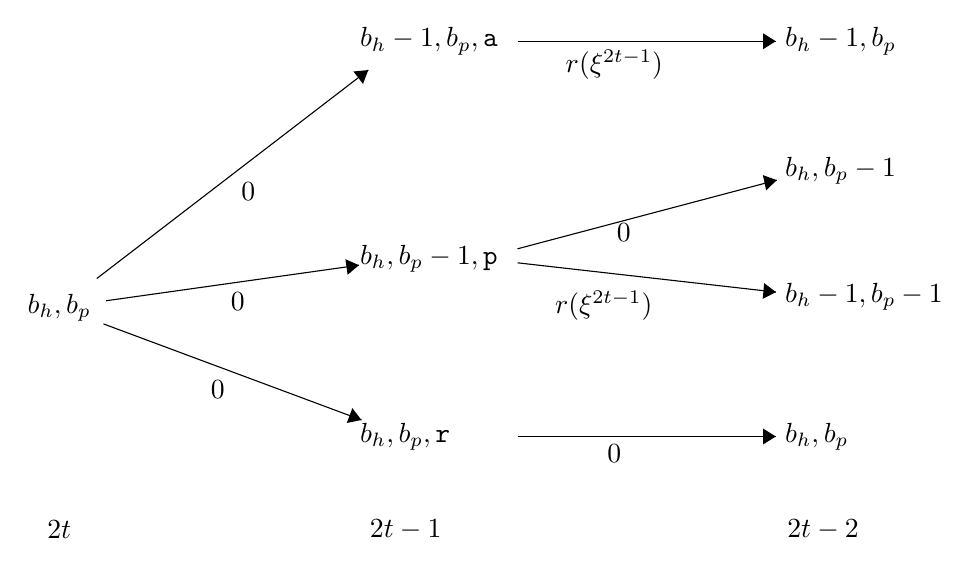
\begin{tikzpicture}[scale=0.2]
\tikzstyle{every node}+=[inner sep=0pt]

\draw (5.9,-25.9) node {$b_h,b_p$};

\draw (5.9,-40) node {$2t$};
\draw (27.9,-40) node {$2t-1$};
\draw (54.4,-40) node {$2t-2$};

\draw (30,-9) node[text width=2cm] {$b_h-1,b_p,\texttt{a}$};
\draw (30,-22.8) node[text width=2cm] {$b_h,b_p-1,\texttt{p}$};
\draw (30,-34.1) node[text width=2cm] {$b_h,b_p,\texttt{r}$};

\draw (57,-9) node[text width=2cm] {$b_h-1,b_p$};
\draw (57,-17.2) node[text width=2cm] {$b_h,b_p-1$};
\draw (57,-34.1) node[text width=2cm] {$b_h,b_p$};
\draw (57,-25.2) node[text width=2cm] {$b_h-1,b_p-1$};


\draw [black] (8.28,-24.07) -- (25.52,-10.83);
\fill [black] (25.52,-10.83) -- (24.58,-10.92) -- (25.19,-11.71);
\draw (17.91,-17.95) node [below] {$0$};
\draw [black] (8.87,-25.48) -- (24.93,-23.22);
\fill [black] (24.93,-23.22) -- (24.07,-22.84) -- (24.21,-23.83);
\draw (17.24,-24.94) node [below] {$0$};
\draw [black] (8.71,-26.95) -- (25.09,-33.05);
\fill [black] (25.09,-33.05) -- (24.51,-32.3) -- (24.16,-33.24);
\draw (15.97,-30.52) node [below] {$0$};

\draw [black] (35,-9) -- (51.4,-9);
\fill [black] (51.4,-9) -- (50.6,-8.5) -- (50.6,-9.5);
\draw (41.15,-9.5) node [below] {$r(\xi^{2t-1})$};
\draw [black] (35,-22.18) -- (51.46,-17.82);
\fill [black] (51.46,-17.82) -- (50.58,-17.5) -- (50.79,-18.47);
\draw (41.75,-20.58) node [below] {$0$};
\draw [black] (35,-23.07) -- (51.41,-24.93);
\fill [black] (51.41,-24.93) -- (50.66,-24.36) -- (50.57,-25.36);
\draw (40.47,-24.83) node [below] {$r(\xi^{2t-1})$};
\draw [black] (35,-34.1) -- (51.4,-34.1);
\fill [black] (51.4,-34.1) -- (50.6,-33.6) -- (50.6,-34.6);
\draw (41.15,-34.6) node [below] {$0$};
\end{tikzpicture}
}
\caption{Transitions for the online probing problem. 
Numbers below the arrows represent the reward of a transition.
At time $2t$ the possible actions are: accept, probe and reject.
At $2t-1$, depending on $\diamond$, we can either accept or reject and $b_h$ may be discounted.
}
\label{fig:probing_states}
\end{figure}




\subsection{Relaxation for Multiple Probing}

The natural relaxation is similar to \cref{eq:probing_relaxation}, but it presents a new challenge.
For binary cases, it was obvious that, if \off wants to probe an arrival, he will always accept it if it is active.
In this case it could be that \off probes $j$ in hope of observing $r_{j2}$ and will reject $r_{j1}$.
We must, therefore, reason about \off's actions at all times, instead of just at even times as before and concluding with structural properties.

Let $\calX\defeq\Rp^{4n}$ be the space for the decision variables.
In \cref{eq:probing_lp} we present a LP which will be the building block for our relaxation.
Note that, by definition, if $t$ is odd, $Z_j(t)=Z_j(t+1)-\In{\xi^{t+1}=j}$.

\begin{equation}\label{eq:probing_lp}
\begin{array}{rrll}
(P[t,Z,b]) \; \max & \multicolumn{3}{l}{\sum_{j,k}r_{jk}(x_{(j,k)a}+q_{jk}x_{ja})} \\
\text{s.t.}& \sum_{j,k}x_{(j,k)a}+\sum_jx_{ja} &\leq b_h  \\
&  \sum_j x_{jp} & \leq b_p   \\
&  x_{ja} +x_{jp} & \leq Z_j(t)  & j\in [n] \\
& x_{(j,k)a} &\leq q_{jk}x_{jp} &  j \in [n],k\in [2]\\ 
& x&\in\calX.
\end{array}
\end{equation}

The LP in \cref{eq:probing_lp} can be interpreted as follows...\todonote

We are ready to parse the relaxation in \cref{eq:probing_relax}.
Recall that a state is of the form $s=(b_h,b_p,\diamond)$ with $\diamond\in \crl{\texttt{a},\texttt{p},\texttt{r},\varnothing}$, where $\diamond=\varnothing$ for even times.
\begin{equation}\label{eq:probing_relax}
\varphi(t,s,\xit) = \left\{ 
\begin{array}{ll}
v(P[t,Z,b]) & \diamond=\varnothing \\ 
v(P[t-1,Z,b]) & \diamond = \texttt{r} \\ 
r_{\xit}+v(P[t-1,Z,b]) & \diamond = \texttt{a} \\ 
\max\crl{r_{\xit}+v(P[t-1,Z,b-e_h]),v(P[t-1,Z,b])} & \diamond = \texttt{p}
\end{array} 
\right.
\end{equation}

\begin{lemma}
Let $\bar X\in\calX$ be a maximizer of $(P[t,Z,b])$ for $t$ even.
Say $\xit=j$, then, at time $t$, \off is satisfied with the following actions:
\begin{enumerate}
\item Accept if $\bar X_{ja}\geq 1$
\item Reject if $\bar X_{ja}+\bar X_{jp}\leq Z_j(t)-1$
\item Probe if $\bar X_{jp}\geq 1$ and then accept $(j,k)$ if $\bar X_{(j,k)a}\geq 1$
\end{enumerate}
\end{lemma}
\begin{proof}
We will show that $\varphi$ satisfies the relaxed Bellman equations, then conclude in virtue of \cref{prop:relaxed_bellman}.
The initial condition follows from the same argument as in \cref{prop:probing_relaxation}.
We are left to show the the probabilistic inequality
\[
\varphi(t,s,\xit) \leq \max_{u\in\U}\crl{R(s,\xit,u)+\E_{\xi^{t-1}}[\varphi(t-1,\Tr(s,\xit,u),\xi^{t-1})|\xit]} \quad \forall \omega\in\calB(t,s).
\]
The set $\calB(t,s)$ is defined as the $\omega\in\Omega$ such that at least one of the conditions (1),(2) or (3) are satisfied.
Observe that, since $t$ is even, the instant reward $R(s,\xit,u)$ is zero.
In cases (1) and (2) is easy to verify the probabilistic inequality.
For case (3) we apply Jensen's Inequality:
\begin{align*}
\varphi(t,s,\xit) &= v(P[t,Z,b]) \\
&= \max\crl{\E[r_{\xi^{t-1}}|\xit]+v(P[t-1,Z,b-e_p-e_h]),v(P[t-1,Z,b-e_p])} \\
&\leq \E_{\xi^{t-1}}[\max\crl{r_{\xit}+v(P[t-1,Z,b-e_h-e_p]),v(P[t-1,Z,b-e_p])}].
\end{align*}
The last term equals $R(s,\xit,u)+\E_{\xi^{t-1}}[\varphi(t-1,s\ominus\texttt{p},\xi^{t-1})|\xit]$ and the proof is complete.
\end{proof}

\section{Stochastic Knapsack With Frequentist Learning}
\paragraph{Problem Statement}
Items with known reward $r$ and random weight $W$ can be placed in a knapsack of capacity $B$.
At every time $t$, an arrival $j\in[n]$ is drawn with some known distribution, which generates a known reward of $r_j$.
The weight $W_j$ is a random variable, which is revealed only after the decision of accept/reject has been made.
The support of $W_j$ is known, but not the distribution.
An arrival can be accepted only if the weight is a.s.\ smaller than the remaining capacity.
At the end of each period, we observe the realization of both accepted and rejected items.

\off has access to the distribution of weights, \emph{but not to the realizations}.
Let $w_j\defeq \E[W_j]$ and $\Wt_j$ be the empirical average of the weights observed.
We assume that, before the process starts, we are given one sample of each weight type to initialize $\hat W_{jt}$.

Let $N_j(t)$ be the number of samples type $j$ observed at the beginning of $t$.
By definition we have $N_j(t)=Z_j(\T)-Z_j(t)+1$.
Following the same arguments, we can show that the relaxation in \cref{eq:knapsack_lp2} satisfies the initial condition.
\begin{equation}\label{eq:knapsack_lp2}
\begin{array}{rrll}
\varphi(t,b,\xit) \; = \; \max & \multicolumn{3}{l}{\sum_{j}r_{j}x_j} \\
\text{s.t.}& \sum_{j} w_jx_j  &\leq b  \\
&  x_j & \leq Z_j(t)  & j\in [n] \\
& x&\geq 0.
\end{array}
\end{equation}

Define as $\hat \varphi(t,b)$ the LP obtained from \cref{eq:knapsack_lp2} by replacing $Z_j(t)$ and $w_j$ by $\mu_j(t)\defeq\E[Z_j(t)]$ and $\Wt_j$, respectively.
Let $\sigma_j\in[n]$ be the rank of $j$ w.r.t.\ the ratio $r_j/w_j$, breaking ties lexicographically. 
For example, if $\sigma_j=1$, it means that $j$ is the most desirable item.
Similarly, $\sigmat_j$ denotes the rank of $j$ w.r.t.\ the ratio $r_j/\Wt_j$.

\begin{lemma}
Assume there are two items ($n=2$)  and $\abs{w_1-w_2}=\Delta>0$.
Let $\Xts,\Xt$ be the solutions to $\varphi,\hat\varphi$ respectively, then
\[
\Pr[\Xt_j\geq \mu_j(t)/2, \Xts<1] \leq STUFF, \quad 
\Pr[\Xt_j< \mu_j(t)/2, \Xts>Z_j(t)-1]\leq STUFF
\]
\end{lemma}
\begin{proof}
Let us bound the first probability by partitioning the space as
\[
\Pr[\Xt_j\geq \mu_j(t)/2, \Xts<1] \leq \Pr[\Xt_j\geq \mu_j(t)/2, \Xts<1, \sigma_j=\sigmat_j] + \Pr[\sigma_j\neq\sigmat_j].
\]
The term $\Pr[\sigma_j\neq\sigmat_j]$ decays with the number of samples $N_1(t),N_2(t)$.
We now bound the other term.

Say $j=1$ and let us study the case $\sigma_1=1$ first.
We can write $\Xts_1 = Z_1(t)\land \frac{b}{w_1}$ and $\Xt_1 = \mu_1(t)\land \frac{b}{\Wt_1}$.
Since we are assuming $\Xt_1\geq \mu_1(t)/2$, it follows that $\frac{b}{\Wt_1}\geq \mu_1(t)/2$.
On the other hand, $\Xts_1<1$ necessitates $\frac{b}{w_1}<1$ or $Z_1(t)=0$.
We can use these two inequalities to conclude
\[
\Pr[\Xt_j\geq \mu_j(t)/2, \Xts<1, \sigma_j=\sigmat_j=1] \leq \Pr[ w_1> \Wt_1 \mu_1(t)/2 \text{ or }  Z_1(t)=0].
\]
The probability of both events decay with $\mu_1(t)$.

Finally, let us study the case $\sigma_1=2$.
We can write $\Xts_2 = Z_2(t)\land \frac{b}{w_2}$, $\Xt_2 = \mu_2(t)\land \frac{b}{\Wt_2}$, $\Xts_1 = Z_1(t)\land \frac{b-\Xts_2w_2}{w_1}$ and $\Xt_1 = \mu_1(t)\land \frac{b-\Xt_2\Wt_2}{\Wt_1}$.
The conditions $\Xt_1\geq \mu_1(t)/2$ and $\Xts_1<1$ imply
\begin{align*}
& \Wt_1\frac{\mu_1(t)}{2}+\Xt_2\Wt_2\leq b < w_1+\Xts_2w_2 \quad \text{ or } \quad Z_1(t)=0\\
&\Longrightarrow \Wt_1\frac{\mu_1(t)}{2}< w_1+ (Z_2(t)w_2)\land b - (\mu_2(t)\Wt_2)\land b \quad \text{ or } \quad Z_1(t)=0 \\
&\Longrightarrow \Wt_1\frac{\mu_1(t)}{2}< w_1+ \abs{Z_2(t)w_2 -\mu_2(t)\Wt_2} \quad \text{ or } \quad Z_1(t)=0.
\end{align*}
For the last implication we used the fact that $x\land b - y\land b \leq \abs{x-y}$ holds for any reals $x,y,b$.
We conclude by observing that both events have probability decaying with $\mu_1(t),N_1(t),N_2(t)$.
\end{proof}

\section{Conclusions}
\input{sec_conclu.tex}


%% Bibliography
\bibliographystyle{plain}
\bibliography{biblio}

\end{document}
